\documentclass[12pt,a4paper]{book}
%Packages used
\usepackage{lipsum}
%Loading images
\usepackage{graphicx}
%For lists
\usepackage{enumitem}
\usepackage{fancyhdr}  % for custom headers and footers
\usepackage{emptypage}
\usepackage{titlesec}
\usepackage[innercaption]{sidecap} % for making side captions to tables/figures
\sidecaptionvpos{figure}{c} % to center side caption vertically wrt the figure
\sidecaptionvpos{table}{c} % to center side caption vertically wrt the table
%\usepackage[document]{ragged2e}
%Margins
\usepackage[left=2.5cm, right=2cm, bottom=2.5cm, top=2cm]{geometry}
%for hyperlinks
\usepackage[colorlinks=true,linkcolor=blue,citecolor=teal]{hyperref}
\usepackage[utf8]{inputenc}
%fonts
\usepackage{amsmath, amssymb, amsfonts}%  for math
\usepackage{bbm}
\usepackage[scaled=0.85]{beramono}%% mono
\usepackage{fourier}
\usepackage[T1]{fontenc}
\usepackage[square,sort&compress,comma,numbers]{natbib}
\usepackage{multirow}
\usepackage{colortbl}
\usepackage{bigstrut}
\usepackage{bm}
\usepackage{array}
\usepackage[table,xcdraw]{xcolor}
\usepackage{float}
\usepackage{physics}
\usepackage{nicefrac}
%No indent
\usepackage[labelfont=bf]{caption} 
\captionsetup[SCfigure]{name={\small \textbf{Figure}}}
\captionsetup[SCtable]{name={\small \textbf{Table}}}
\usepackage{parskip}
\usepackage{alphabeta}

\newcolumntype{C}[1]{>{\centering\arraybackslash}p{#1}}
\renewcommand{\arraystretch}{1.25} % increasing height of the rows

\newcommand{\unchapter}[1]{%
  \begingroup
  \let\@makechapterhead\@gobble % make \@makechapterhead do nothing
  \chapter{#1}
  \endgroup
}
\makeatother

% chapter title format
\titleformat{\chapter}[display]
  {
  \normalfont\LARGE\raggedleft
}
  {\hspace*{\fill} \chaptertitlename \ \thechapter }
  {0pt}
  {\hspace*{\fill} \Huge\bfseries} [\hrulefill  \vspace{-1.0cm}]

% chapter title format (for special cases when no space above the chapter title is desired)
\newcommand{\highchapter}[1]{%
  \begingroup
  \titleformat{\chapter}[display]
    {
    \normalfont\LARGE\raggedleft
    }
    {}
    {0pt} % Adjusts vertical space ABOVE the title (negative moves it higher)
    {\vspace*{-3cm} \hspace*{\fill} \Huge\bfseries} 
    [\vspace{-0.5cm} \rule{\textwidth}{1.5pt} \vspace{-2.2cm}] % Custom thick rule
  \chapter*{#1}
  \endgroup
}

% Set up fancyhdr
\pagestyle{fancy}
\fancyhf{}  % Clear all header and footer fields
% Odd pages: Italicized chapter number and title
\fancyhead[RO]{\itshape \leftmark}
% Even pages: Italicized section number and title
\fancyhead[LE]{\itshape \rightmark}
% Centered page numbers in the footer
\fancyfoot[C]{\thepage}
% Ensure no horizontal rules
\renewcommand{\headrulewidth}{0.4pt}  % Line under the header
\renewcommand{\footrulewidth}{0pt}  % No line above the footer
% Redefine \chaptermark and \sectionmark to include numbers and italics in headers
\renewcommand{\chaptermark}[1]{\markboth{\itshape Chapter \thechapter .\ \ #1}{}}
\renewcommand{\sectionmark}[1]{\markright{\itshape \thesection\ \ #1}}

% Setting up background filling for caption boxes
% Define the background color
\definecolor{captionbg}{RGB}{230,230,230}
% Set a small margin between the caption text and box boundaries
\setlength{\fboxsep}{3pt}  % Adjust the padding inside the box
% Customizing the captions
\DeclareCaptionFormat{myformat}{
    \colorbox{captionbg}{\parbox{\dimexpr\linewidth-2\fboxsep}{#1#2#3}}
}
\captionsetup{
    format=myformat,  % Apply the custom format
    skip=3pt          % Adjust extra space between figure/table and its caption
}

% Figure and Table labels in bold
\makeatletter
\renewcommand{\fnum@figure}{\small \textbf{Figure \thefigure}}
\renewcommand{\fnum@table}{\small \textbf{Table \thetable}}
\makeatother

% depth of the table of contents tree
\setcounter{tocdepth}{1}

\makeatletter
% Redefine the \tableofcontents to add custom formatting for the TOC title
\renewcommand{\tableofcontents}{%
  \highchapter{Table of Contents} % Unnumbered chapter for the TOC title
  \setlength{\parskip}{-6pt} % Remove space between paragraphs
  \@starttoc{toc} % Start the table of contents itself
}

% by adjusting \vskip one can play with the space between the TOC lines
\renewcommand*\l@chapter[2]{%
    \ifnum \c@tocdepth >\m@ne \addpenalty {-\@highpenalty }\vskip 8pt \@plus \p@ \setlength \@tempdima {1.5em}
    \begingroup \parindent \z@ \rightskip \@pnumwidth \parfillskip -\@pnumwidth \leavevmode \bfseries \advance \leftskip \@tempdima \hskip -\leftskip #1\nobreak \hfil \nobreak \hb@xt@ \@pnumwidth {\hss #2\kern -\p@ \kern \p@ }\par \penalty \@highpenalty \endgroup \fi}

% Redefine the \listoffigures command to add custom formatting for the title
\renewcommand{\listoffigures}{%
  \highchapter{\listfigurename} % Unnumbered chapter for list of figures title
  \@starttoc{lof} % Start the list of figures
}

% Redefine the \listoftables command to add custom formatting for the title
\renewcommand{\listoftables}{%
  \highchapter{\listtablename} % Unnumbered chapter for list of tables title
  \@starttoc{lot} % Start the list of tables
}

\renewenvironment{thebibliography}[1]{%
  \highchapter{\bibname}
  \addcontentsline{toc}{chapter}{Bibliography}
  \small
  \list{\@biblabel{\@arabic\c@enumiv}}%
    {\settowidth\labelwidth{\@biblabel{#1}}%
     \leftmargin\labelwidth
     \advance\leftmargin\labelsep
     \setlength{\itemsep}{0pt} % Remove extra space between items
     \setlength{\parskip}{0pt} % Remove extra space between paragraphs
     \usecounter{enumiv}%
     \let\p@enumiv\@empty
     \renewcommand\theenumiv{\@arabic\c@enumiv}}%
  \sloppy\clubpenalty4000\widowpenalty4000%
  \sfcode`\.\@m
}{%
  \endlist
  \normalsize
}

\makeatother

\begin{document}

%Useful formatting:
% \\ for newline without paragraph
% \par for newline with paragraph
%To import and generate code for tables you may, for example, use: https://www.tablesgenerator.com/

\thispagestyle{empty}
\newgeometry{left=3cm,bottom=0.1cm}

%----- title page -----
%Do not alter this page, only fill out the required fields
\begin{figure}
\vspace{-1.5cm}

\includegraphics[width=0.15\columnwidth]{logo/University_of_Luxembourg_logo_(fr).png}
\centering
\end{figure}

\begin{center}
\footnotesize{PhD-No PhD-FSTM-2025-xxx }\\
%\vspace{0.4cm}
\footnotesize{The Faculty of Science, Technology and Medicine}\\
\vspace{1.0cm}
\Large{DISSERTATION}\\
\vspace{1.0cm}
\normalsize{Presented on xx/xx/2025 in Luxembourg}\\
\vspace{0.25cm}
\normalsize{to obtain the degree of}\\
\vspace{1.0cm}
\Large{DOCTEUR DE L'UNIVERSITÉ DU LUXEMBOURG}\\
\vspace{0.5cm}
\Large{EN PHYSIQUE}\\
\vspace{0.5cm}
by\\
\vspace{0.5cm}
\Large{Name SURNAME}\\
\vspace{0.25cm}
\normalsize{Born on date in place (country)}\\
\vspace{1.0cm}
    \Large{\MakeUppercase{My Thesis Title Here}}

{\raggedright
\vspace{1.0cm}
\Large{Dissertation defense committee}\\
\vspace{0.25cm}
\normalsize{Dr. John Jones, Supervisor}\\
\textit{Professor, University}\\
\vspace{0.25cm}
\normalsize{Dr. Martin Martins, Chairman }\\
\textit{Professor, University}\\
\vspace{0.25cm}
\normalsize{Dr. David Davidson, Vice-Chairman}\\
\textit{Professor, University}\\
\vspace{0.25cm}
\normalsize{Dr. Christian Christensen}\\
\textit{Professor, University}\\
\vspace{0.25cm}
\normalsize{Dr. James Jameson}\\
\textit{Professor, University}\\
\vspace{0.25cm}
}
\end{center}

\newpage
\restoregeometry

\thispagestyle{empty}

%----- empty -----
\newpage \ \newpage

%----- Dedications -----
\newpage
\thispagestyle{empty}
\begin{center}
\vspace*{\fill}
\raggedleft
\textit{
`` And yet it moves!'' \\ Galileo Galilei \\ (optional)
}
\end{center}
\vspace*{\fill}
\newpage

% Abstract
%\pagenumbering{roman} 
\frontmatter
\highchapter{Abstract}
\addcontentsline{toc}{chapter}{Abstract}
% your abstract here
\input{sections/abstract}
\markboth{}{} %end chapter

%\chapter*{Acknowledgments}
%\addcontentsline{toc}{chapter}{Acknowledgments}
% your abstract here
%\input{sections/acknowledgements}
%\markboth{}{} %end chapter

%----- empty -----
%\newpage \ \newpage

%----- preface -----
\highchapter{Preface}
\addcontentsline{toc}{chapter}{Preface}
\noindent {\Large{\bf{Acknowledgements}}} \\

Acknowledgements

\newpage
\noindent {\Large{\bf{Note on publications}}} \\

This thesis builds upon and incorporates material from the following (published) papers:

\begin{enumerate}[label={\arabic*.}]
\item First paper.
\item Second paper.
\end{enumerate} 

\markboth{}{} %end chapter

%----- table of contents -----
{
  \hypersetup{linkcolor=black}
  \tableofcontents
}
\addcontentsline{toc}{chapter}{Table of Contents}
\markboth{}{} %end chapter

%----- list of abbreviations -----
\highchapter{List of Abbreviations}
\addcontentsline{toc}{chapter}{List of Abbreviations}
%\printacronyms[name=]
\begin{tabular}{cp{1.0\textwidth}}
  \textbf{DFT}            & Density Functional Theory \\
  \textbf{HF}             & Hartree-Fock \\
  \textbf{QM}		        & Quantum Mechanics \\
  \textbf{(RS)PT}		    & (Rayleigh-Schr{\"o}dinger) Perturbation Theory \\
\end{tabular}\\
\newpage \ \newpage
%----- empty -----

%----- list of symbols -----
\highchapter{List of Symbols and Notation}
\addcontentsline{toc}{chapter}{List of Symbols and Notation}
\begin{tabular}{cp{0.9\textwidth}}
  $\nabla_{\mathbf{r}}$		    & gradient operator: $\left(\frac{\partial}{\partial x},\frac{\partial}{\partial y},\frac{\partial}{\partial z}\right)^T$ \\
  $\int d\mathbf{r}$		    & integral over three-dimensional space: $\int \int \int dx\,dy\,dz$ \\
  $\hat{H}$           & Hamiltonian operator \\
  $k_e$               & Coulomb constant: $k_e = 1/4\pi\varepsilon_0$ \\
  $m$                 & (effective) mass \\
  $q$                 & (effective) charge \\
  $\mathbf{T}$        & dipole-dipole coupling tensor \\
\end{tabular}\\
\newpage \ \newpage

%----- list of figures -----
%\chapter*{List of Figures}
{
  \hypersetup{linkcolor=black}
  \listoffigures 
}
\newpage
\addcontentsline{toc}{chapter}{List of Figures}
\markboth{}{} %end chapter

%----- list of tables -----
%\chapter*{List of Tables}
{
  \hypersetup{linkcolor=black}
  \listoftables 
}
\newpage
\addcontentsline{toc}{chapter}{List of Tables}
\markboth{}{} %end chapter
\newpage \ \newpage

\mainmatter
%----- introduction -----
\chapter{Introduction}
\label{intro}
\addtocontents{lof}{\protect\contentsline{chapter}{\numberline{\thechapter} Introduction}{}{}}
\addtocontents{lof}{\vspace{6pt}}
Introduction

The famous Schr{\"o}dinger equation
\begin{equation}
    i\hbar \frac{\partial \psi}{\partial t} = \hat{H}\psi
\label{eq: SE}
\end{equation}
was proposed in Ref.~\cite{Schrodinger1926}.
\addtocontents{lof}{\vspace{-6pt}}

%----- chapter 2 -----
\chapter{Chapter 2 title}
\addtocontents{lof}{\protect\contentsline{chapter}{\numberline{\thechapter} Chapter 2}{}{}}
\addtocontents{lof}{\vspace{6pt}}
\label{chapter2}
Text of the Chapter 2.

\section{First subsection}

\begin{SCfigure}[1.0][h]
    \centering
    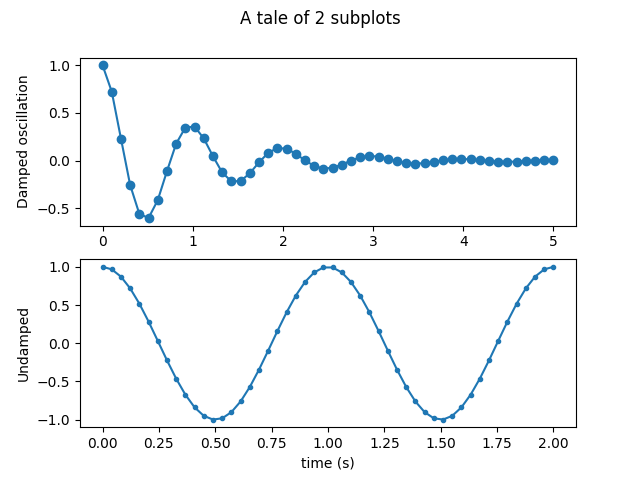
\includegraphics[width=0.7\linewidth]{imgch2/mpl-example.png}
    \caption[Short caption for TOC]{Full caption to the figure with explanations.}
    \label{fig: fig1}
\end{SCfigure}

\vskip 2cm

\begin{SCtable}[][h]
    \centering
    \begin{tabular}{|c|c|}
    \hline
         \pi & 3.1415926 \\
         $e$ & 2.718281828 \\
    \hline
    \end{tabular}
    \caption{Table caption}
    \label{tab: tab1}
\end{SCtable}
\addtocontents{lof}{\vspace{-6pt}}

%----- chapter 3 -----
\chapter[Chapter 3 short title for TOC]{Chapter 3 full title}
\addtocontents{lof}{\protect\contentsline{chapter}{\numberline{\thechapter} Chapter 3}{}{}} \addtocontents{lof}{\vspace{6pt}}
\addtocontents{lot}{\protect\contentsline{chapter}{\numberline{\thechapter} Chapter 3}{}{}} \addtocontents{lot}{\vspace{6pt}}
\label{chapter3}
{\raggedleft \textit{Parts of this chapter have been published in this or similar form in:} \\
reference to a paper.\\}

\hrulefill 

Reference to Eq.~\eqref{eq: SE} from Chapter~\ref{intro}.
\addtocontents{lof}{\vspace{-6pt}}
\addtocontents{lot}{\vspace{-6pt}}

%----- chapter 4 -----
\chapter{Chapter 4 title}
\addtocontents{lof}{\protect\contentsline{chapter}{\numberline{\thechapter} Chapter 4}{}{}}
\addtocontents{lof}{\vspace{6pt}}
\addtocontents{lot}{\protect\contentsline{chapter}{\numberline{\thechapter} Chapter 4}{}{}} \addtocontents{lot}{\vspace{6pt}}
\label{chapter4}
\input{sections/chapter4}
\addtocontents{lof}{\vspace{-6pt}}
\addtocontents{lot}{\vspace{-6pt}}

%----- chapter conclu -----
{\chapter{Summary and Outlook}
\label{conclusions}
\input{sections/conclusions}
\markboth{}{} %end chapter
%----- empty -----
}
 
{%----- appendix -----
\chapter*{Appendices}
\addcontentsline{toc}{chapter}{Appendices}
\addtocontents{lof}{\protect\contentsline{chapter}{Appendices}{}{}} \addtocontents{lof}{\vspace{6pt}}
\addtocontents{lot}{\protect\contentsline{chapter}{Appendices}{}{}} \addtocontents{lot}{\vspace{6pt}}
\renewcommand\thesection{A\arabic{section}}
\renewcommand\thesubsection{A\arabic{subsection}}
\setcounter{figure}{0}
\setcounter{table}{0}

\renewcommand{\thetable}{{A\arabic{table}}}
\renewcommand{\thefigure}{{A\arabic{figure}}}
\renewcommand{\theequation}{{A\arabic{equation}}}

\subsection{Appendix}

Appendix A1.

\subsection{Appendix}

Appendix A2.
\addtocontents{lof}{\vspace{-6pt}}
\markboth{}{} %end chapter
}


{%----- References -----
\bibliography{biblio.bib}
\bibliographystyle{apsrev4-1.bst}
%----- empty -----
}

\end{document}